\documentclass[8pt]{beamer}
\usepackage[utf8]{inputenc}

\usetheme{Madrid}

%% ADDITIONAL NICOLÁS
\usepackage{ragged2e}
\usepackage{amssymb}
\usepackage{subcaption}

\usefonttheme{serif}
\definecolor{UBCblue}{rgb}{0.01569, 0.11765, 0.25882} % PSU Blue
\usecolortheme[named=UBCblue]{structure}

%% ADDITIONAL NICOLÁS


\newcommand{\locx}{\mathbf{x}}
\newcommand{\vele}{\mathbf{e}_\alpha}

%------------------------------------------------------------
%This block of code defines the information to appear in the
%Title page
\title[Simulation Reports] %optional
{PhD in Energy and Mineral Engineering at PSU}

\subtitle{Nicolás's Research - Reports}

\author[Nicolás Bueno] % (optional)
{Nicolás Bueno\inst{1} \and Advisor: Dr. Ayala\inst{1}}

\institute[EME] % (optional)
{
	\inst{1}%
	Department of Energy and Mineral Engineering\\
	Penn State University\\
	
\includegraphics[height=1cm]{pics/PSU_EMS.png}
}

\date[Spring 2022] % (optional)
{}

%\logo{
\includegraphics[height=1cm]{pics/PSU_EMS.png}}

%End of title page configuration block
%------------------------------------------------------------



%------------------------------------------------------------
%The next block of commands puts the table of contents at the 
%beginning of each section and highlights the current section:

\AtBeginSection[]
{
	\begin{frame}
		\frametitle{Table of Contents}
		\tableofcontents[currentsection]
	\end{frame}
}
%------------------------------------------------------------


\begin{document}
	
	%The next statement creates the title page.
	\frame{\titlepage}
	
	%---------------------------------------------------------
	%This block of code is for the table of contents after
	%the title page
	\begin{frame}
		\frametitle{Table of Contents}
		\tableofcontents
	\end{frame}
	%---------------------------------------------------------
	%---------------------------------------------------------
	\justifying
	\section{Rising droplet - Partition coefficient}
	
	\subsection*{Considerations}
	\label{}
	\justifying
	\begin{frame}[t]{Considerations}
		\justifying
		
		
		\begin{columns}[t]
			
			\column{0.45\textwidth}
			\textbf{Considerations}\\~\\
			\justifying
			
			Goal: Test the pseudopotential approach for partially misc. mixtures, under the action of a second force.\\~\\
			
			Idea: test different flow regimes based on Reynolds and Bond (Eotvos) numbers, and capture particular bubble shapes, as found by Flit R, Grace JR, Weber M. \textit{Bubbles, drops, and particles}. New York: Academic Press; 1978. 
			
			\begin{equation*}
			R_e = \frac{\rho_l u_b d_b}{\mu_l} = \frac{u_b d_b}{\nu_l}
			\end{equation*}
			\begin{equation*}
			B_o = \frac{g \Delta \rho d_b^2}{\sigma}
			\end{equation*}
			
			\column{0.45\textwidth}{
			\justifying
			
			}
			
			A thermodynamic state fixes $\rho, \Delta \rho, \sigma$. Redifining $R_e$:
			\begin{equation*}
				Re = \frac{d_b \sqrt{g d_b} }{\nu_l} =  \frac{\sqrt{g d_b^3}}{\nu_l}
			\end{equation*}
			
			We can sweep the spectrum by fixing $g$ (fixes $B_o$), and moving $\nu_l$ (fixes $R_e$), as:
			\begin{equation*}
				\nu_l = c_s^2 (\tau_l - \frac{\Delta t}{2})
			\end{equation*}
				
			\begin{equation*}
				\begin{split}
					g = \frac{B_o \sigma}{\Delta \rho d_b^2}\\
					\nu_l = \frac{\sqrt{g d_b^3}}{R_e}\\
					\tau_l = \frac{\nu_l}{c_s^2}+ \frac{\Delta t}{2}
				\end{split}
			\end{equation*}
		\end{columns}
	\end{frame}
	
	\subsection*{Initial setup}
	\begin{frame}[t]{Initial setup}
		\justifying
		\begin{columns}[t]
			\column{0.45\textwidth}
			
			\textbf{Domain}: (!) 300x300 mesh (2D)\\
			\textbf{Fluid}: Water at 485.33 K ($T_r$ = 0.75), and $P_r$ = 0.092. \\$\rho_l^0$  = 7.679 (), $\rho_v^0$  = 0.109. $\rho_r$ = 70.45.\\
			Initial condition: Spherical droplet with $d_o$ = 30, and $w_o$ = 8.
			
			~\\
			\textbf{Boundary conditions}: The top and bottom boundaries are PERIODIC. On the left and right boundaries a no-slip condition is imposed. At the corners, where there is a PDF that may belong to two boundaries, the enumeration and assignation of conditions is as follows:
			\begin{itemize}
				\item Corner 1 (SW): No-slip (Left)
				\item Corner 2 (NW): No-slip (Left)
				\item Corner 3 (SE): No-slip (Right)
				\item Corner 4 (NE): No-slip (Right)
			\end{itemize}
		

			
			
			\column{0.45\textwidth}
			
			\textbf{Parameters}: Shan-Chen $G$=-1.0. \\
			Beta = 0.2076\\
			Time = 100000\\
			
			~\\
			\textbf{Single static simulation}:\\ $\Delta \rho $ = 7.59285, $d_s$ = 29.45, \\ $\Delta P$ = 0.00378 ($P_l < 0$). \\$\sigma$ = 0.1112.
		\end{columns}
	\end{frame}


	\subsection*{Initial setup 2 (Amaya)}
	\begin{frame}[t]{Initial setup 2 (Amaya)}
		\justifying
		\begin{columns}[t]
			\column{0.45\textwidth}
			
			\textbf{Domain}: (!) 160x400 mesh (2D)\\
			\textbf{Fluid}: Water at 485.33 K ($T_r$ = 0.75), and $P_r$ = 0.092. \\$\rho_l^0$  = 7.679 (), $\rho_v^0$  = 0.109. $\rho_L/\rho_g$ = 70. $\tau_l$ = 210.5. $\tau_g$ = 0.8. $\mu_l/\mu_g$ =10.\\
			Initial condition: Spherical droplet with $d_o$ = 40, and $w_o$ = 8.
			
			~\\
			\textbf{Boundary conditions}: Periodic on all boundaries (for static), walls on all boundaries (for dynamic). At the corners, where there is a PDF that may belong to two boundaries, the enumeration and assignation of conditions is as follows:
			\begin{itemize}
				\item Corner 1 (SW): No-slip (Left)
				\item Corner 2 (NW): No-slip (Left)
				\item Corner 3 (SE): No-slip (Right)
				\item Corner 4 (NE): No-slip (Right)
			\end{itemize}
			
			
			
			
			\column{0.45\textwidth}
			
			\textbf{Parameters}: Shan-Chen $G$=-1.0. \\
			Beta = 0.2076\\
			Time = 100000\\
			
			~\\
			\textbf{Single static simulation}:\\ $\Delta \rho $ = 7.2 (7.7-0.5), $d_s$ = 40.0, \\ $\Delta P$ = 8.5e-3 - 5.87e-3 = 2.623e-3 \\$\sigma = \Delta P \cdot r$ = 0.05254.
			$B_o$ =10. Then, $g = \frac{\sigma B_o}{\Delta \rho d^2}$ = 4.5e-5. $\mu_l $ = 0.85, $\nu_l$ = 0.1105. $\tau_l$ = 0.83.  
		\end{columns}
	\end{frame}

	%---------------------------------------------------------
	%---------------------------------------------------------
	\subsection*{Results}
	\begin{frame}[t]{Spherical regime}
		\textbf{}\\~\\
		
		First case (150 x 300)
		\begin{itemize}
			\item $g = \vert \mathbf{g}\vert $ = -1e-6. $B_o$ = 0.0592. $\tau_l$ = 2.0, $\nu$ = 0.5. $u_b$ = 0.0121. 
			\item $R_e^{\text{org}}$ = 0.713. $R_e^{\text{mod}}$ = 0.320. 
			
			\item This is spherical regime, and far away from the other regimes according to the Grace's plot. 
		
		\end{itemize}
		
	\end{frame}
	
	\begin{frame}[t]{Ellipsoidal case}
		Ellipsoid case (150 x 300)
		\begin{itemize}
			\item $g = \vert \mathbf{g}\vert $ = -1e-5. $B_o$ = 0.592. $\tau_l$ = 0.51, $\nu$ = 0.0033. $u_b \approx$ = 0.35. 
			\item $R_e^{\text{org}}$ = 3092. $R_e^{\text{mod}}$ = 151.61
			\item This simulation is approaching to the Mach velocity limit and a perturbation is moving the bubble from the axis. I decided to open the channel more to avoid the interaction with the wall. I have reasons to believe that the movement beyond the axis is due to whom the corner was assigned to (number of boundary).
		\end{itemize}
		Ellipsoid case (300 x 300)
		\begin{itemize}
			\item $g = \vert \mathbf{g}\vert $ = -1e-5. $B_o$ = 0.592. $\tau_l$ = 0.51, $\nu$ = 0.0033. $u_b \approx$ = 0.35. 
			\item $R_e^{\text{org}}$ = 3092. $R_e^{\text{mod}}$ = 151.61
			
			\item The ellipse shape of the bubble was better seen in this case, although eventually it moves away from the center. For the most part of the simulation, the ellipsoid maintains, although it is important to understand if the viscosity of the gas phase plays any role in the deformation ("plasticity" of the bubble).
			
			\item Apr 15/22. The ellipse is not moving anymore from the center. 
		\end{itemize}
	\end{frame}

	\begin{frame}[t]{Dimples}
			
		Dimples case (300 x 300)
		\begin{itemize}
			\item $g = \vert \mathbf{g}\vert $ = -2e-3. $B_o$ = 118 $\tau_l$ = 0.72, $\nu$ = 0.07348. $u_b \approx$ = . 
			\item $R_e^{\text{org}}$ = . $R_e^{\text{mod}}$ = 100
			\item The gravity value is too high and the method is diverging too soon. Not even with G = -0.1 or g = 1e-4.
		\end{itemize}	
	
		Dimples case (3000 x 3000)
		\begin{itemize}
		\item $d_o$ = 300. $g = \vert \mathbf{g}\vert $ = -1e-5. $B_o$ = 61. $\tau_l$ = 0.993, $\nu$ = 0.164 $u_b \approx$ = . 
		\item $R_e^{\text{org}}$ = . $R_e^{\text{mod}}$ = 100
		\item Did not run
	\end{itemize}	
	Dimples case (3000 x 3000)
		\begin{itemize}
			\item $d_o$ = 300. $g = \vert \mathbf{g}\vert $ = -1e-5. $B_o$ = 61. $\tau_l$ = 5.43, $\nu$ = 1.64 $u_b \approx$ = . 
			\item $R_e^{\text{org}}$ = . $R_e^{\text{mod}}$ = 10
			\item Did not run
		\end{itemize}		
	\end{frame}


	\section{New forcing scheme}
	
	\begin{frame}{Forcing scheme}
	Taking advantage of the mutual interactions between components, 
	the pseudopotential is accounting only for attraction between components, while an extra term accounts for the usual repulsion term:
	\begin{equation*}
	\begin{split}
	F_i^\sigma =  - \frac{1}{c_s^2 \delta t} \sum_\alpha  w_\alpha  e_{\alpha,i} [\frac{R_sT}{1-b_m \rho} - c_s^2 ] \rho_\sigma ( \locx + \vele \delta t) \\ - \psi^\sigma \sum_{\sigma_2} G_{\sigma,\sigma_2} \sum_\alpha w_\alpha e_{\alpha,i} \psi^{\sigma_2} ( \locx + \vele \delta t)  
	\end{split}
	\end{equation*}
	
	Where $\psi$ and $G_{\sigma,\sigma_2}$ are defined as:
	\begin{equation}
		\begin{split}
		\psi^\sigma = \rho^\sigma \sqrt{\frac{a^\sigma}{f(b\rho)}}\\
		G_{\sigma,\sigma_2} = \frac{2(\varLambda_{\sigma, \sigma_2}-1)}{c_s^2 \delta t} 
		\end{split}
	\end{equation}
	where $f(b\rho)$ is the density-dependent polynomial in the denominator of the attraction term in the cubic equation of state. Here, the terms $a,b$ are given in mass-basis, so proper conversions must be taken care of. 
	\end{frame}

	\begin{frame}{Taylor Expansion}
		
		Generic form:
		\begin{equation*}
		F_i = \sum_\alpha T (\locx + \vele \delta t)  w_\alpha \vele
		\end{equation*}
		
		Replacing the Taylor expansion of $T$
		\begin{equation*}
		\begin{split}
		F_i = 
		T(\mathbf{x}) \sum_\alpha w_\alpha \vele + \partial_j T \delta t \sum_\alpha w_\alpha \vele\vele^j + \frac{\delta t^2}{2} \partial_j \partial_k (T) \sum_\alpha w_\alpha \vele \vele^j \vele^k + \\\frac{\delta t^3}{6} \partial_j \partial_k \partial_l (T) \sum_\alpha w_\alpha \vele \vele^j \vele^k \vele^l 
		\end{split}
		\end{equation*}
		
		Continuum approach: \begin{equation*}\label{eq:taylorExpansion}
		\begin{split}
		F_i = c_s^2 \delta t  \partial_i T  + \frac{c_s^4\delta t^3}{2} \partial_i \partial_{kk} (T) 
		\end{split}
		\end{equation*}
		
		Resulting pressure;
		\begin{equation*}\label{eq:pressureLBMPseudoP}
		\begin{split}
		p = c_s^2 \sum_\sigma \rho_\sigma + \frac{c_s^2 \delta t}{2} \sum_\sigma \sum_{\sigma_2} G_{\sigma,\sigma_2} \psi_\sigma \psi_{\sigma_2} + \sum_\sigma   (\frac{R_sT}{1-b_m \rho} - c_s^2) \rho_\sigma \\ p =  \frac{R_sT}{(1-b_m \rho)} \rho - \frac{a_m \rho^2}{f(b_m \rho)}
		\end{split}
		\end{equation*}
	\end{frame}

	\section{1D comparision of splitting scheme and new scheme}
	\begin{frame}{Simulation setup}
		
		\begin{columns}
			
			\column{0.5\textwidth}
			From van der Waals implementation into the phase behavior model (C++):\\~\\
			
			Name, mw, pc, tc, acen, vc, shift\\
			C3 0.044097 615.8 666.05 0.1522 0.0 0.0\\
			C5 0.044097 488.5 845.80 0.2514 0.0 0.0\\~\\
			
			Conditions:\\
			P = 275.36 psi, T = 192.34 F. z = [0.5, 0.5]\\~\\
			
			Results from flash:
			
			Densities = 13.5852 lb/ft3, 2.3956 lb/ft3 (4.693187 lu, 0.8275917 lu)\\
			Fugacities = 906.34 kPa, 604.423 kPa (0.043939432 lu, 0.029302344 lu)\\
			Liquid composition = [0.36357, 0.63643]\\
			Gas composition = [0.54527, 0.45473]\\
			Ki = 1.49975, 0.714505. $\gamma$ = 0.642
			\column{0.5\textwidth}
			
		\end{columns}
		
	\end{frame}


	\begin{frame}{Results}
		The density profile converges to the correct values given by the vdW EoS. The splitting coefficient, with no calibration in $\beta$, compromises the vapor density to under predicted values.
		\begin{figure}
			\centering
			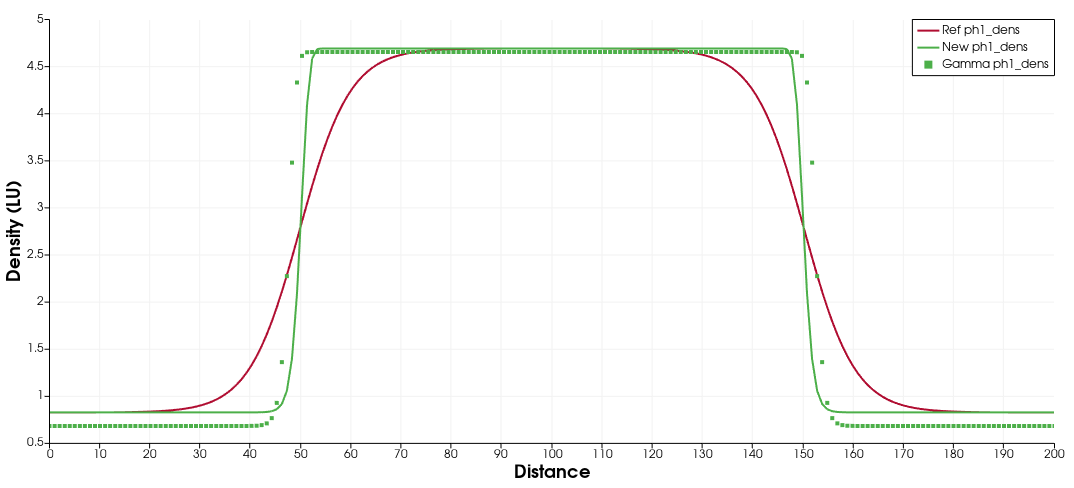
\includegraphics[width=\textwidth]{pics/1dnewForce/density.png}
		\end{figure}
	\end{frame}
	
	\begin{frame}{Results}
		The pressure with the new scheme converges to the correct pressure value. The splitting scheme, as the density of the vapor is lower, the convergence pressure is also lower. Due to the small compressibility of the liquid, to achieve this value of pressure, small changes in density are needed, so the liquid density is not compromised.
		\begin{figure}
			\centering
			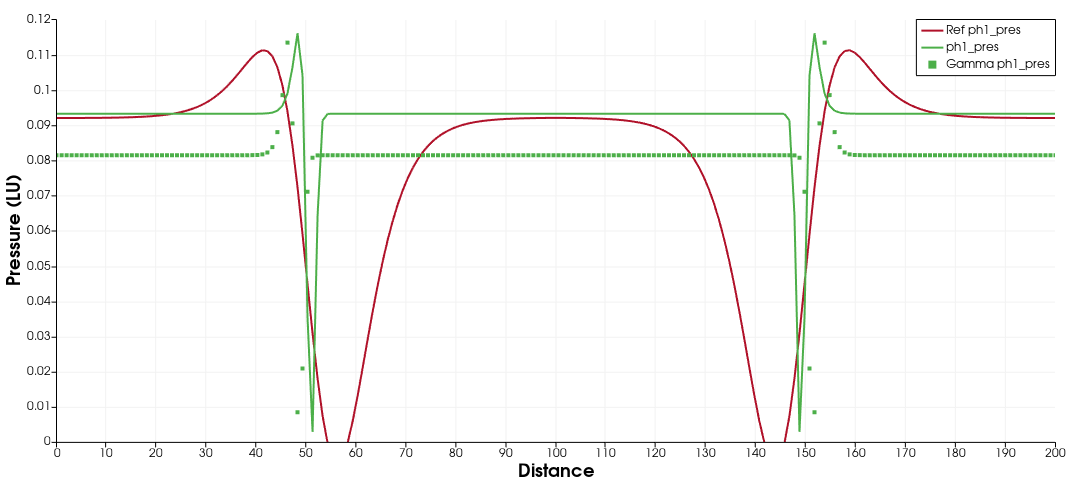
\includegraphics[width=\textwidth]{pics/1dnewForce/pressure.png}
		\end{figure}
	\end{frame}

	\begin{frame}{Results}
		The compositions in both cases do not match with equilibrium values. This is due that the model does not allow for diffusion if the pressure is already in equilibrium. These results suggest that transport is favored to keep the liquid properties are they were initialized, and balances the vapor properties accordingly.
		\begin{figure}
			\centering
			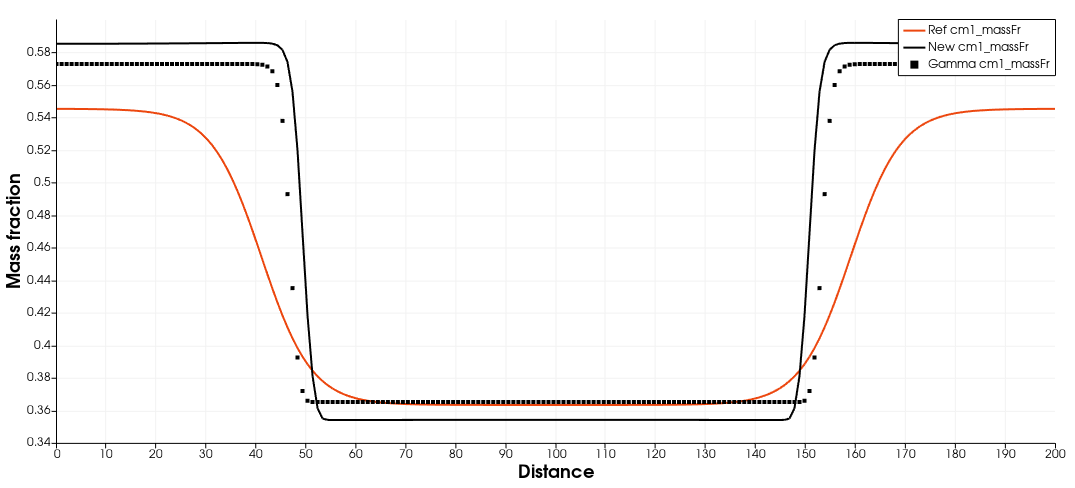
\includegraphics[width=\textwidth]{pics/1dnewForce/massFraction.png}
		\end{figure}
	\end{frame}

	\begin{frame}{Results}
		Fugacities prove the non chemical-equilibrium in the system.
		\begin{figure}
			\centering
			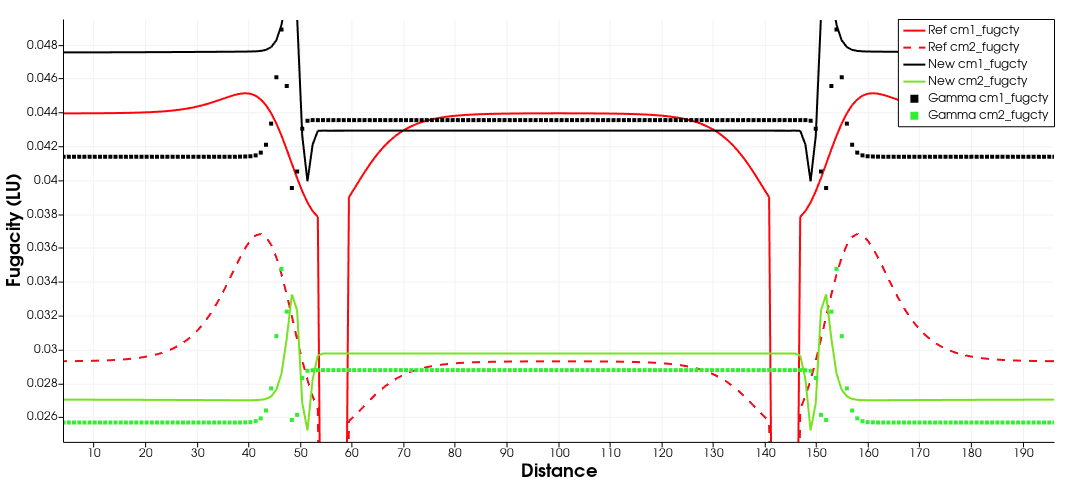
\includegraphics[width=\textwidth]{pics/1dnewForce/fugacity.png}
		\end{figure}
	\end{frame}

	\begin{frame}{Results}
		\begin{figure}
			\centering
			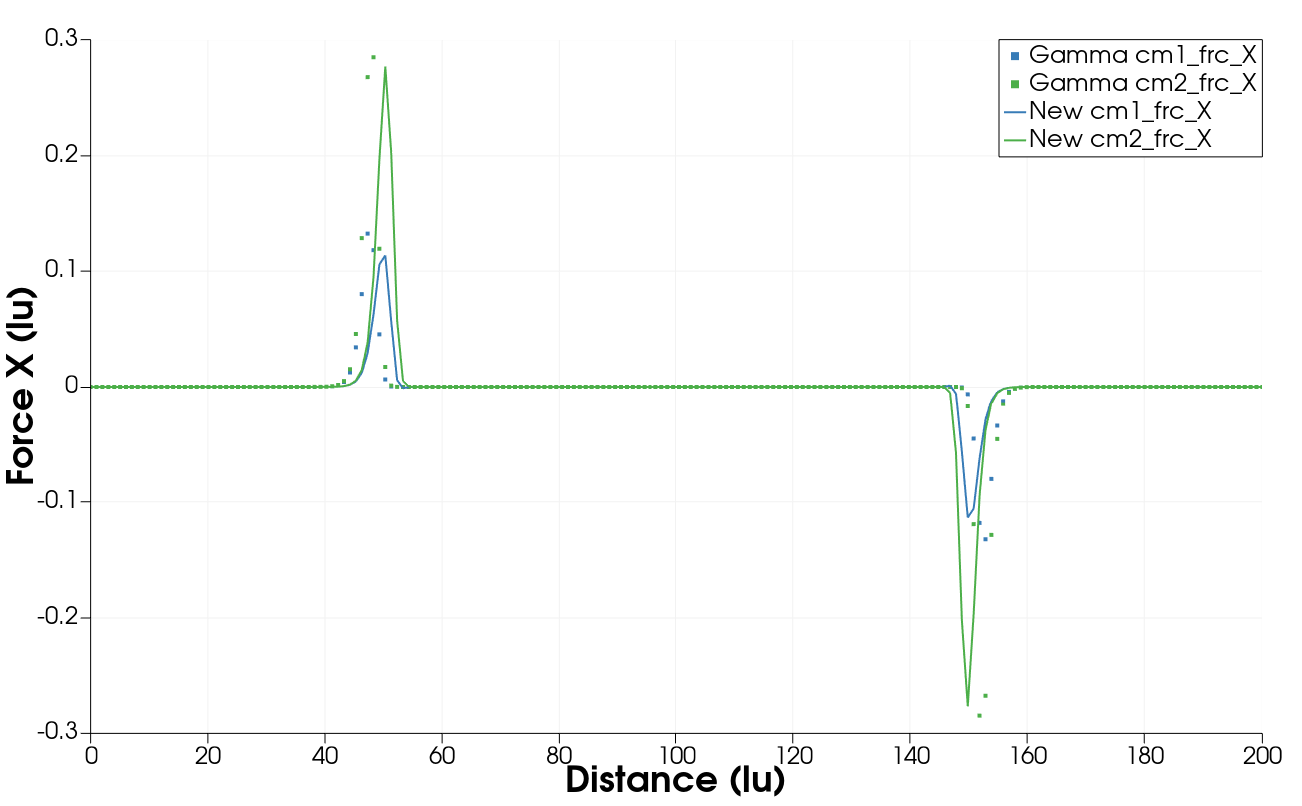
\includegraphics[width=\textwidth]{pics/1dnewForce/forceX.png}
		\end{figure}
	\end{frame}

	
	%---------------------------------------------------------
	%---------------------------------------------------------
	\section{2D rising bubble simulation}
	\begin{frame}{Simulation setup}
		\justifying
		\begin{columns}[t]
			\column{0.45\textwidth}
			
			\textbf{Domain}: 160x400 mesh (2D)\\
			\textbf{Fluid}: C3 and C5
			\begin{tabular}{|c|c|c|c|}
				\hline
				Acentric & Tc & Pc & Mw \\
				\hline
				0.1522 & 370 & 42.46 & 0.044097 \\
				\hline
				0.2514 & 469.9 & 33.68 & 0.072150 \\
				\hline
			\end{tabular}
		
			Temperature 362.0 K (Tr = 0.83). 
			
			Equilibrium conditions: $\rho_l, \rho_v$ (lbm/ft3) = 31.89, 1.86. $mw_l, mw_v$ (g/mol) = 61.95, 51.88. $\bar{\rho}_\text{ratio}$ = 14.32. $K_1, K_2$ = 1.987, 0.436. $\gamma$ = 0.583. 
			
			.\\
			
			~\\
			\textbf{Boundary conditions}: Full periodic.
			\textbf{Initial conditions}: Time 10000. Bubble in thermodynamic equilibrium, $r_0, w_0$ = .
			
			
			
			\column{0.45\textwidth}
			Two models were tested: new forcing scheme, and the Sankarana model.
			
			\textbf{Parameters}: Shan-Chen $G$=-1.0. \\
			Beta = 0.2076\\
			Time = 100000\\
			
			~\\
			\textbf{Single static simulation}:\\ $\Delta \rho $ = 7.59285, $d_s$ = 29.45, \\ $\Delta P$ = 0.00378 ($P_l < 0$). \\$\sigma$ = 0.1112.
			
		\end{columns}
	\end{frame}
	
	\begin{frame}[t]{Results Sankarana}
		In this model, the pseudopotential is given by $\psi_1 = \sqrt{\frac{\rho_1}{1-b_1\rho_1}- a_1 \rho^2_1 - \rho_2}$ and $\psi_2 = \rho_2$\\~\\

		Initialization: $\rho_l$ = 5.75, $\rho_v$ = 2.17. $z_{1,l}$ = 0.98, $z_{1,v}$ = 0.48. $r_e$ = 24.5, $w$ = 5.0.\\~\\

		Static results:\\
		$\rho_l$ = 5.77, $\rho_v$ = 2.18. $z_{1,l}$ = 0.98, $z_{1,v}$ = 0.53. For $r_e$ = 27, $\Delta p = \frac{\sigma}{r}$ = 0.00274. $\sigma$ = 0.074.

		\begin{equation*}
			\begin{split}
			B_o = \frac{g \Delta \rho d_b^2}{\sigma} = 141.465e3 \cdot g\\
			M_o = \frac{g \Delta \rho \mu_l^4}{\sigma^3 \rho_l^2} = \frac{g \Delta \rho \nu_l^4 \rho_l^2}{\sigma^3} = 294.952e3 \cdot g \cdot \nu^4_l
			\end{split}
		\end{equation*}

	\end{frame}



	\begin{frame}{}
		
	\end{frame}

	\begin{frame}
	\end{frame}
	%---------------------------------------------------------
	\section*{Useful frame options}
	\label{}
	\justifying
	\begin{frame}
		\textbf{Report XXX XX - 202X}\\~\\
		Main discussion points:
		\begin{itemize}
			\item Topic 1
			\item Topic 2
		\end{itemize}
	\end{frame}

	\begin{frame}{Discussion}
		\begin{columns}
			
			\column{0.5\textwidth}
			
			
			\column{0.5\textwidth}
			
		\end{columns}
	\end{frame}
	%---------------------------------------------------------
	%---------------------------------------------------------
	\begin{frame}
	\end{frame}
	%---------------------------------------------------------
	%---------------------------------------------------------
	\begin{frame}
	\end{frame}
	%---------------------------------------------------------
	%---------------------------------------------------------
	\begin{frame}
	\end{frame}
	%---------------------------------------------------------
		%---------------------------------------------------------
	%Changing visivility of the text
	\begin{frame}
		\frametitle{Sample frame title}
		This is a text in second frame. For the sake of showing an example.
		
		\begin{itemize}
			\item<1-> Text visible on slide 1
			\item<2-> Text visible on slide 2
			\item<3> Text visible on slides 3
			\item<4-> Text visible on slide 4
		\end{itemize}
	\end{frame}
	
	%---------------------------------------------------------
	
	
	%---------------------------------------------------------
	%Example of the \pause command
	\begin{frame}
		In this slide \pause
		
		the text will be partially visible \pause
		
		And finally everything will be there
	\end{frame}
	%---------------------------------------------------------
	
	%---------------------------------------------------------
	%Highlighting text
	\begin{frame}
		\frametitle{Sample frame title}
		
		In this slide, some important text will be
		\alert{highlighted} because it's important.
		Please, don't abuse it.
		
		\begin{block}{Remark}
			Sample text
		\end{block}
		
		\begin{alertblock}{Important theorem}
			Sample text in red box
		\end{alertblock}
		
		\begin{examples}
			Sample text in green box. The title of the block is ``Examples".
		\end{examples}
	\end{frame}
	%---------------------------------------------------------
	
	
	%---------------------------------------------------------
	%Two columns
	\begin{frame}
		\frametitle{Two-column slide}
		
		\begin{columns}
			
			\column{0.5\textwidth}
			This is a text in first column.
			$$E=mc^2$$
			\begin{itemize}
				\item First item
				\item Second item
			\end{itemize}
			
			\column{0.5\textwidth}
			This text will be in the second column
			and on a second tought this is a nice looking
			layout in some cases.
		\end{columns}
	\end{frame}
	%---------------------------------------------------------
	
	
\end{document}